\chapter{Effekt ECS}\label{chap:engine}

In this chapter, we will go over the general concept and usage of our game engine implementation and its API.

For our game engine library, visibility via namespaces was not feasible, as some |interface|s had internal and accessible operations, and it would be very time-consuming to change this for our library. We instead chose to prefix the internal effect operations with |internal_...|, so it would also be clear that the developer using the library should not call these.

\section{General Differences}

Comparing to existing ECS implementations, our version is an archetype based ECS and does not use chunks to store components for the same archetype. It uses effects to model all the different parts a complete ECS needs, building up from simple ones.

The ECS uses a |Component| effect to model the component storage of all instances of a single component type. Each entity then has a (potentially different) component index for each of its components, which is not very typical for existing ECSs. Details about this system are explained in \Cref{sec:compimpl}. This often results in non-sequential iteration of components during runtime, which is not very efficient at memory access. Although this memory inefficiency should not make a very big difference on the \textsf{js-web} target, as we discuss in more detail in \Cref{sec:indirectaccess}.

Component queries are also implemented differently to most other ECSs. We have a |Query| effect that can be defined as a named effect handler. Inside a system, the query iteration operation on the |Query| handler can then be called, which iterates over all queried entities. Onto a |Query| handler, different components and filters can be added. When a component (including optional ones) is added to the query, a new named handler of the |CompIter| effect gets defined. Inside the |Query| iteration loop, the current component from each of the |CompIter| handlers can be retrieved and modified with the respective |get| and |set| effect operations. This is explained in more detail and with examples in \Cref{sec:queries}.

\section{World and Engine}

\newcommand\Engine[1]{
  \node[box,minimum height=5cm,minimum width=4cm] at (0,#1) {};
  \node[] at (0,#1+2.25) {engineWorld};
  \node[box,fill=yellow!20,minimum height=0.5cm,minimum width=3cm] at (0,#1+1.5) {Position};
  \node[box,fill=yellow!20,minimum height=0.5cm,minimum width=3cm] (enginecomp) at (0,#1+1) {Rotation};
  \node[box,fill=yellow!20,minimum height=0.5cm,minimum width=3cm] at (0,#1+0.5) {Scale};
  \node[box,fill=purple!20,minimum height=0.5cm,minimum width=3cm] at (0,#1-0.25) {RunWorld};
  \node[box,fill=purple!20,minimum height=0.5cm,minimum width=3cm] (engineres) at (0,#1-0.75) {Time};
  \node[box,fill=purple!20,minimum height=0.5cm,minimum width=3cm] at (0,#1-1.25) {TimeScale};
  \node[box,fill=blue!10,minimum height=0.5cm,minimum width=3cm] (enginesys) at (0,#1-2) {Time \& Exit System};
  \draw[->] ([yshift=-0.25cm] enginecomp.west) -- node[near start,anchor=north] {register} ([yshift=0.2cm] comp.east);
  \draw[->] ([yshift=-0.25cm] engineres.west) -- node[near start,anchor=north] {register} ([yshift=0.2cm] res.east);
  \draw[->] (enginesys.west) -- node[near start,anchor=north] {register} ([yshift=0.2cm] sys.east);
}

\newcommand\Canvasrenderer[1]{
  \node[box,minimum height=4cm,minimum width=4cm] at (0,#1) {};
  \node[] at (0,#1+1.75) {canvasRenderer};
  \node[box,fill=yellow!20,minimum height=0.5cm,minimum width=3cm] (rendercomp) at (0,#1+1) {Shape};
  \node[box,fill=yellow!20,minimum height=0.5cm,minimum width=3cm] at (0,#1+0.5) {DrawHeight};
  \node[box,fill=purple!20,minimum height=0.5cm,minimum width=3cm] (renderres) at (0,#1-0.25) {Camera};
  \node[box,fill=purple!20,minimum height=0.5cm,minimum width=3cm] at (0,#1-0.75) {WindowProperties};
  \node[box,fill=blue!10,minimum height=0.5cm,minimum width=3cm] (rendersys) at (0,#1-1.5) {Render System};
  \draw[->] ([yshift=-0.25cm] rendercomp.west) -- node[near start,anchor=north] {register} (comp.east);
  \draw[->] ([yshift=-0.25cm] renderres.west) -- node[near start,anchor=north] {register} (res.east);
  \draw[->] (rendersys.west) -- node[near start,anchor=north] {register} (sys.east);
}

\newcommand\Input[1]{
  \node[box,minimum height=1cm,minimum width=4cm] (input) at (-8,#1) {};
  \node[] at (-8,#1) {Input Module};
  \draw[->] (ecs.north) -- node[midway,anchor=west] {init} (input.south);
}

\newcommand\Gamemodule[1]{
  \node[box,minimum height=4cm,minimum width=4cm] at (0,#1) {};
  \node[] at (0,#1+1.75) {Game (example)};
  \node[box,fill=yellow!20,minimum height=0.5cm,minimum width=3cm] (gamecomp) at (0,#1+1) {Velocity};
  \node[box,fill=yellow!20,minimum height=0.5cm,minimum width=3cm] at (0,#1+0.5) {Health};
  \node[box,fill=purple!20,minimum height=0.5cm,minimum width=3cm] (gameres) at (0,#1-0.25) {PauseState};
  \node[box,fill=blue!10,minimum height=0.5cm,minimum width=3cm] (gamesys) at (0,#1-1) {Move System};
  \node[box,fill=blue!10,minimum height=0.5cm,minimum width=3cm] at (0,#1-1.5) {Healing System};
  \draw[->] ([yshift=-0.25cm] gamecomp.west) -- node[near start,anchor=north] {register} ([yshift=-0.2cm] comp.east);
  \draw[->] (gameres.west) -- node[near start,anchor=north] {register} ([yshift=-0.2cm] res.east);
  \draw[->] ([yshift=-0.25cm] gamesys.west) -- node[near start,anchor=north] {register} ([yshift=-0.2cm] sys.east);
}

\begin{figure}[h!]
\centering
\tikzstyle{box}=[rectangle,draw,rounded corners=0.5ex,fill=green!10]
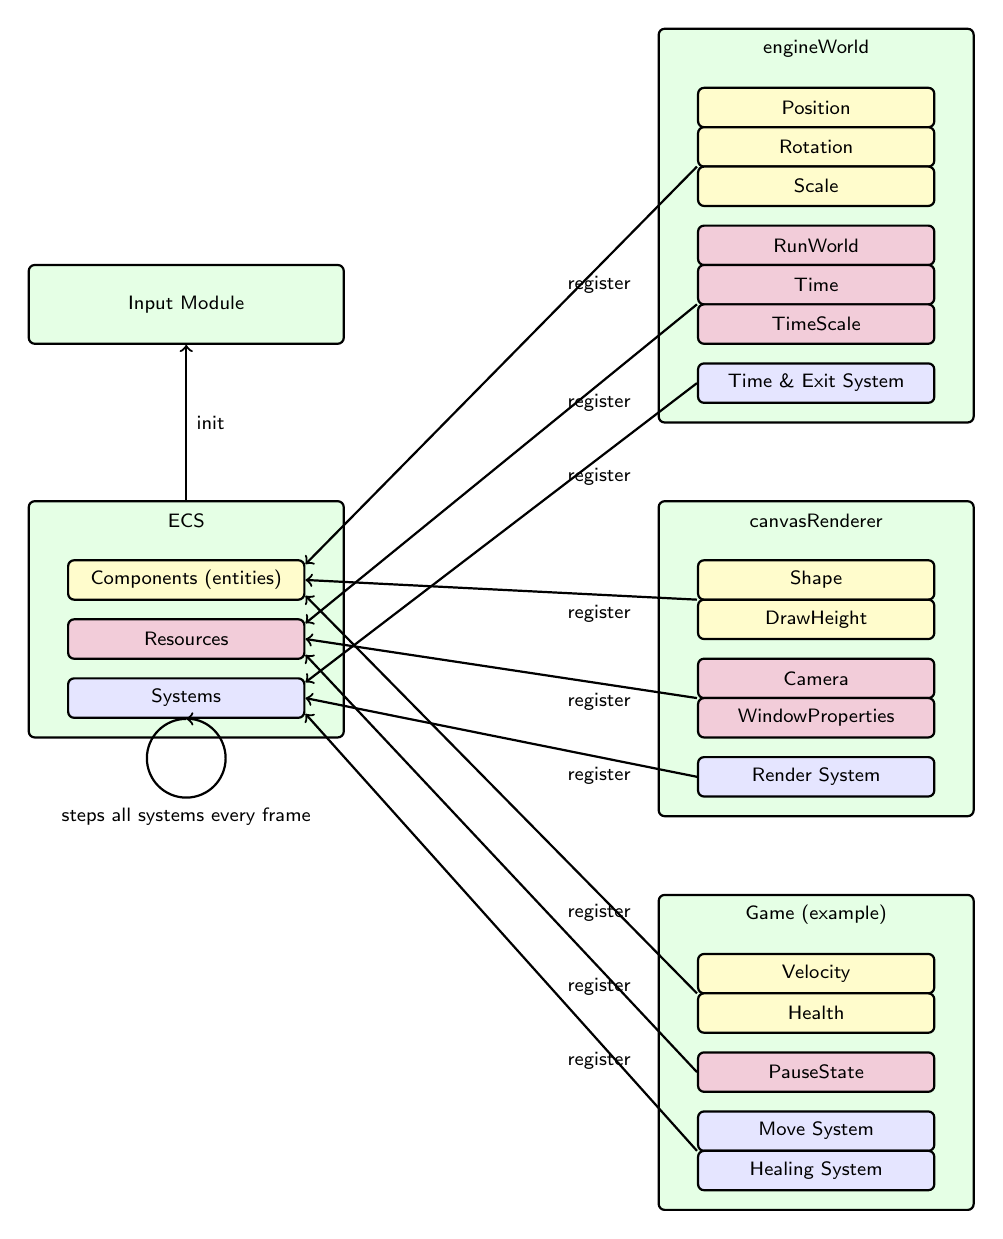
\begin{tikzpicture}[thick,font=\sf\scriptsize]
  \node[box,minimum height=3cm,minimum width=4cm] (ecs) at (-8,0) {};
  \node[] at (-8,1.25) {ECS};
  \node[box,fill=yellow!20,minimum height=0.5cm,minimum width=3cm] (comp) at (-8,0.5) {Components (entities)};
  \node[box,fill=purple!20,minimum height=0.5cm,minimum width=3cm] (res) at (-8,-0.25) {Resources};
  \node[box,fill=blue!10,minimum height=0.5cm,minimum width=3cm] (sys) at (-8,-1) {Systems};
  \draw[->] (sys.south) arc (90:450:5mm) node[midway,anchor=north] {steps all systems every frame};
  \Engine{5}
  \Canvasrenderer{-0.5}
  \Input{4}
  \Gamemodule{-5.5}
\end{tikzpicture}
\caption{Structure of the Effekt game engine. The \textit{Game} module is an example of how the game logic is added to the engine.}
\label{fig:effektengine}
\end{figure}

To use the ECS, the |World| effect must first be handled. The engine has some additional code around the ECS that creates basic resources and systems every game needs, as seen in \Cref{fig:effektengine}. By using this |engineWorld| function to initialize the engine, it will also automatically create a |World| effect handler first. If those resources and systems should not be needed, the |world| function can be used directly. Additionally, any needed modules can be initialized/added after handling a |World| by calling their initialization functions. One of these modules is the |canvasRenderer| that is currently needed for any graphical game.

\begin{lstlisting}
with engineWorld();
with canvasRenderer();
\end{lstlisting}

The |World| effect is used to hold all systems and run them in order. As it also represents the base structure of the developed ECS, the |world| function, which handles the |World| effect, also handles all of the internal effects that are needed by the ECS. This includes the |ComponentManager|, |ArchManager|, |EntityIdManager|, |EntityManager| and a resource that can be toggled to exit the game loop inside the world. Most of these are explained more thoroughly in \Cref{chap:details}. Calling the |runWorld| effect operation of the |World| effect (|do runWorld();|) starts the game loop, executing all systems in order every frame, until the escape key is pressed.

Once a |World| has been handled, any modules and game code can be added to it by creating queries and adding systems which use these queries to the |World|. Some basic resources and systems get created by the |engineWorld| function, which include |Time|, |TimeScale| and their update system, as seen in \Cref{fig:effektengine}. It also resets the per-frame keyboard inputs from the input module using the \textit{ffi} and exits the game loop on pressing the escape key. Other modules like the |canvasRenderer| add their components, resources and systems similarly. The game code by the game developer does the same as well after initialization; Creating components, resources and adding systems to the |World| using queries.

\section{Components and Resources}

The |Component[T]| effect defines a component storage for the engine internals to store, get and set components of any single type. A handler for any type of components can be created with the |component| function. After registering, the component type can be used in all functions that need the |Component[T]| effect, for example adding it to entities.

\begin{lstlisting}
record Velocity(value: Vector2)
record Health(value: Int)
record EnemyTag()

def main() = {
  ... // Init engine
  with component[Velocity]();
  with component[Health]();
  with component[EnemyTag]();
}
\end{lstlisting}

The |Resource[T]| effect is very straightforward. When creating a resource with the |resource| function, an inital value must be provided, and that resource is then available to |get| or |set| at any time. This serves as single values that may be needed by multiple systems and should not be connected to any entity.

\section{Queries and Systems}\label{sec:queries}

\textit{Queries} are used to iterate collections of specific components that can further filter which entities are included or excluded. The previous code snippet demonstrates how to create a |Query| using all its available effect operations to iterate specific components and to filter by additional ones. Handling the |Query| effect with the |query| function and binding it to a name creates an ''empty query'', meaning it will iterate over every entity without accessing any components. After that, specific (optional) components can be added to the query by calling the |addC| or |addOptC| effect operations on the previously created query. With these operations, a |CompIter| effect handler can be bound to a name, which is used during iteration of the query to |get| or |set| that component of the current entity. To filter the query additionally, the |withC| or |withoutC| effect operations can be called on the query, which will not bind any additional effect handlers. All the |withC| components must also be present on an entity to be iterated by this query and all the |withoutC| components must be absent. These filtered components are not iterated over; they serve only as filters to which entities get queried.

\begin{lstlisting}
with def query = query();
with def velocities = query.addC[Velocity]();
with def optPositions = query.addOptC[Position]();
query.withC[Health]();
query.withoutC[EnemyTag]();
\end{lstlisting}

Systems are added to the |World| by calling the |system| function, which handles the |System| effect while using the |World| effect. These systems take a code block that gets called every frame, in the order the systems are added. Inside this system block, queries can be used to iterate over entities with specific components. An example of adding a system to the |World| and using our previously created query inside it to modify matching entities can be seen in the following code snippet.

\begin{lstlisting}[caption=System example for gravity]
... // Create query
with system() {
  val deltaTime = (do getResource[Time]()).deltaTime;
  // Iterate query, ignoring actual "Entity" values
  query.foreach() { (_) =>
    // Update y-axis velocity
    var velocity = velocities.get().value;
    velocity = velocity + Vector2(0.0, -9.81 * deltaTime);
    velocities.set(Velocity(velocity));
    // When position exists, modify it using velocity
    positions.get() match {
      case Some(position) => positions.set(
        Some(Position(position.value + velocity * deltaTime))
      )
      case None() => ()
    };
  };
}
\end{lstlisting}

This example system will apply gravity and change the position from its velocity if a position exists. This is done for every entity with |Health| that is not an enemy, which could for example match all players and allied characters, but not enemies.

\section{Entity Manager}

The |EntityManager| effect gets automatically handled when using the |world| or |engineWorld|, as it is a core part of the ECS internals. It can be used to create and destroy entities and remove components from them. It can also be used to set components (or add when it is not yet present) and get the current value of components. It also has operations available to check if an entity exists or if it has a specific component. Using the |EntityManager| to create an entity returns the newly created |Entity|'s value, which can for example be stored in a component on another entity to reference it. Most of the other operations, like |setComponent| also need an |Entity| as argument, to which the operation is applied.

Inside all systems, the |EntityManager| effect is overwritten by a different handler to make deferred modification possible for structural changes (create/destroy entities and add/remove components). This ensures there is no modification during iteration, which could lead to an infinite loop or remove components that are yet to be iterated. Other operations, like getting a component, only work if the entity already exists and immediately has the given component on it. These are not deferred and just passed to the outer |EntityManager| handler.
